\documentclass[conference]{IEEEtran}
\IEEEoverridecommandlockouts

% ── Idioma y codificación ──
\usepackage[utf8]{inputenc}
\usepackage[T1]{fontenc}
\usepackage[spanish,es-nodecimaldot,es-noshorthands]{babel}

% ── Paquetes de la plantilla oficial IEEE (+ booktabs para tablas) ──
\usepackage{cite}
\usepackage{amsmath,amssymb,amsfonts}
\usepackage{graphicx}
\usepackage{booktabs}
\usepackage{multirow}
\usepackage{textcomp}
\usepackage{xcolor}

% ── Macros ──
\newcommand{\zb}{z_b}
\newcommand{\RMSE}{\mathrm{RMSE}}
\newcommand{\NRMSE}{\mathrm{NRMSE}}
\newcommand{\pd}[2]{\frac{\partial #1}{\partial #2}}
\newcommand{\TODO}[1]{\textcolor{red}{[\textbf{Pendiente:} #1]}}

\begin{document}

\title{Operador inverso amortizado e informado por física para
inversión de batimetría desde campos de oleaje:\\
generalización fuera de distribución por dificultad}

\author{
\IEEEauthorblockN{Etienne Calderón}
\IEEEauthorblockA{Departamento de Informática\\
Universidad Técnica Federico Santa María\\
Valparaíso, Chile\\
etienne@watermind.space}
\and
\IEEEauthorblockN{Nombre del Profesor Guía}
\IEEEauthorblockA{Departamento de Informática\\
Universidad Técnica Federico Santa María\\
Valparaíso, Chile\\
correo@usm.cl}
}

\maketitle

\begin{abstract}
La batimetría (la profundidad del fondo) modula la propagación del oleaje
superficial a través de las ecuaciones de aguas someras (SWE), lo que en
principio permite invertir la profundidad a partir de observaciones de la
superficie. Los enfoques recientes basados en redes neuronales informadas por
física (PINN) ajustan un modelo por cada escenario, lo que impide evaluar
\emph{generalización} a batimetrías no vistas. Este trabajo plantea la inversión
como el aprendizaje de un \textbf{operador inverso amortizado}: un único modelo
convolucional que mapea el campo espaciotemporal de superficie y velocidad
$(\eta, u)$ a la batimetría $\zb(x)$, entrenado sobre una distribución de fondos.
Sobre este encuadre se introducen tres contribuciones: (i) el operador
amortizado, que recupera una nueva batimetría con una sola pasada hacia adelante;
(ii) un protocolo de evaluación \emph{fuera de distribución (OOD) por dificultad}
junto a un banco de pruebas realista de oleaje incidente en aguas profundas
(inspirado en fiordos del sur de Chile) con ejes de excitación tipo marea; y
(iii) el estudio del residuo SWE como regularizador y su efecto sobre la
generalización OOD. El operador recupera batimetrías de prueba más difíciles
que cualquiera de entrenamiento con un $\RMSE$ de $\sim$1\,cm (frente a
$\sim$1.7\,mm in-distribution), una brecha de generalización de $\approx$5.7$\times$.
Sobre este banco, un regularizador físico ligero (el residuo de continuidad)
mejora la generalización OOD del operador pequeño de forma modesta pero
consistente ($\approx$3\%), y evidencia preliminar indica que aumentar la
capacidad (operador mediano, $5.3\times$ parámetros) también ayuda ($\approx$14\%
mejor en OOD). El límite dominante sigue siendo la complejidad batimétrica: el
error es plano hasta un umbral de dificultad y luego crece de forma abrupta (el
decil más difícil $\approx$5.5$\times$ el más fácil).
\end{abstract}

\begin{IEEEkeywords}
inversión de batimetría, redes neuronales informadas por física, ecuaciones de
aguas someras, aprendizaje de operadores, generalización fuera de distribución.
\end{IEEEkeywords}

% =====================================================================
\section{Introducción}
\label{sec:intro}

El conocimiento de la batimetría es fundamental para la navegación, la
modelación de marejadas e inundaciones, la ingeniería costera y la acuicultura.
Su levantamiento directo (ecosondas multihaz, LiDAR batimétrico) es costoso y
de cobertura limitada, en especial en zonas someras, remotas o de difícil
acceso como los fiordos del sur de Chile. Una alternativa es la
\emph{inversión}: inferir el fondo a partir de observaciones de la superficie
del agua, aprovechando que la dinámica del oleaje somero depende de la
profundidad.

Esta dependencia está descrita por las ecuaciones de aguas someras (SWE): la
celeridad de una onda gravitatoria es $c=\sqrt{gh}$, de modo que la profundidad
queda codificada en cómo el oleaje se refracta, acelera y dispersa sobre el
fondo. Las redes neuronales informadas por física (PINN)~\cite{raissi2019} han
sido aplicadas a esta inversión~\cite{dazzi2024,tian2025,ohara2024}, imponiendo
las SWE como restricción blanda en la función de pérdida. Sin embargo, el
encuadre habitual ajusta \emph{un modelo por cada escenario}: la red se optimiza
para reproducir un único campo observado, recuperando la batimetría de ese caso.
Bajo este esquema no es posible plantear la pregunta de \emph{generalización}
(qué tan bien recupera el modelo batimetrías que no vio), porque cada modelo
sólo ha visto un fondo.

Este trabajo reencuadra la inversión como el aprendizaje de un \textbf{operador
inverso amortizado}: un único modelo que mapea el campo de observaciones
$(\eta(x,t), u(x,t))$ a la batimetría $\zb(x)$, entrenado sobre una
\emph{distribución} de batimetrías. ``Amortizado'' alude a que el costo de
inversión se paga una vez en el entrenamiento, y una nueva batimetría se recupera
luego con una sola pasada hacia adelante, sin reoptimizar. Crucialmente, este
encuadre permite separar entrenamiento y prueba y, con ello, medir generalización.

Las contribuciones son tres:
\begin{enumerate}
  \item Un \textbf{operador inverso amortizado} campo$\to$campo para inversión
        de batimetría desde SWE, en contraste con el ajuste PINN por caso.
  \item Un \textbf{protocolo de evaluación fuera de distribución (OOD) por
        dificultad} y un banco de pruebas sintético \emph{realista}: oleaje
        incidente sobre un dominio abierto de aguas profundas, con ejes de
        excitación tipo marea (amplitud y nivel medio), motivado por la
        aplicación en fiordos.
  \item Un \textbf{estudio del residuo SWE como regularizador físico} y su
        efecto sobre la generalización OOD, es decir, si ``informar por física''
        ayuda a extrapolar a batimetrías más difíciles que las de entrenamiento.
\end{enumerate}

% =====================================================================
\section{Trabajo relacionado}
\label{sec:related}

\paragraph*{Inversión de batimetría con PINN}
Dazzi~\cite{dazzi2024} y Tian \emph{et al.}~\cite{tian2025} invierten batimetría
resolviendo las SWE con PINN; O'Hara~\cite{ohara2024} y trabajos
afines~\cite{chen2023,liu2024} exploran formulaciones y regularizaciones. Estos
enfoques ajustan un campo por caso y reportan la calidad de reconstrucción de
ese caso, sin un protocolo de generalización a batimetrías nuevas.

\paragraph*{Redes informadas por física y embeddings}
Las PINN~\cite{raissi2019} imponen el residuo de la EDP en la pérdida; los
\emph{Fourier features}~\cite{tancik2020} mitigan el sesgo espectral en la
representación de campos. Aquí el residuo SWE se reutiliza como regularizador,
pero evaluado por diferencias finitas sobre los campos observados en lugar de
por diferenciación automática sobre las coordenadas de una red de coordenadas.

\paragraph*{Solvers de aguas someras}
El \emph{ground truth} se genera con esquemas \emph{well-balanced} de volúmenes
finitos~\cite{audusse2004,leveque2002} validados contra soluciones analíticas
clásicas~\cite{thacker1981,delestre2013}, lo que permite generar pares
(batimetría, campo de oleaje) para fondos arbitrarios sin solución cerrada.

% =====================================================================
\section{Metodología}
\label{sec:method}

\subsection{Operador inverso amortizado}
Se busca aprender un operador $\mathcal{G}_\theta$ tal que
$\hat\zb(x) = \mathcal{G}_\theta\big(\eta(x,t), u(x,t)\big)$, entrenado sobre una
distribución de batimetrías $\{\zb^{(n)}\}$ con sus campos de oleaje asociados.
A diferencia del ajuste por caso, el operador procesa el \emph{campo completo}
de observaciones de una vez y, una vez entrenado, invierte un fondo nuevo con un
único \emph{forward pass}.

\subsection{Generación de datos: solver SWE 1D}
El \emph{ground truth} se obtiene resolviendo las SWE 1D transitorias sobre
topografía,
\begin{align}
  \pd{h}{t} + \pd{(hu)}{x} &= 0, \label{eq:swe-cont}\\
  \pd{(hu)}{t} + \pd{}{x}\!\Big(hu^2 + \tfrac{1}{2}gh^2\Big)
    &= -\,g\,h\,\pd{\zb}{x}, \label{eq:swe-mom}
\end{align}
con $h$ la profundidad, $u$ la velocidad, $\eta = h+\zb$ la superficie libre y
$g=9.81$\,m/s$^2$, mediante un esquema \emph{well-balanced} aumentado de tipo
Riemann~\cite{audusse2004}. El solver se valida reproduciendo la cuenca oscilante
de Thacker ($\RMSE$ de $h$ del $0.62\%$ del calado máximo) y preservando el
estado de reposo a precisión de máquina.

\paragraph{Régimen de oleaje incidente}
El forzamiento modela un \emph{tramo abierto de fiordo}: un tren de olas entra
de forma continua por un borde y sale por el opuesto (\emph{outflow}
transmisivo). El borde de entrada usa una condición dependiente del tiempo que
inyecta el oleaje como onda simple mediante los invariantes de Riemann
$R^\pm = u \pm 2\sqrt{gh}$ (el invariante entrante se prescribe y el saliente se
extrapola del interior), de modo que las olas internas abandonan el dominio casi
sin reflejarse. Frente a un dominio cerrado de paredes, que genera resonancias
dependientes del tamaño de la caja que el operador podría memorizar, aquí la
única retro-dispersión proviene de la batimetría: la señal que persiste
\emph{es} interrogación del fondo. La señal inyectada es una superposición de
$1$ a $3$ componentes sinusoidales con rampa suave,
\begin{equation}
  \delta\eta_{\text{in}}(t) = \tanh(t/\tau)\sum_m A_m
    \sin\!\Big(\tfrac{2\pi t}{T_m}+\phi_m\Big),
  \label{eq:wave}
\end{equation}
con períodos largos $T_m\in[5,9]$\,s, fijados por el criterio hidrostático de
la Sección~\ref{sec:fisica} (y que además evitan frentes tipo \emph{bore}), y
rampa $\tanh$ con $\tau\in[2,4]$\,s.

\paragraph{Ejes de excitación tipo marea}
Un único factor latente de sicigia--cuadratura $f\sim\mathcal{U}(0,1)$ (la
posición en el ciclo quincenal de la marea) gobierna de forma coherente ambos
ejes de marea, muestreado de manera idéntica en todos los niveles de dificultad
(ortogonal al eje batimétrico): la \emph{etapa de marea} (nivel medio)
$\ell = \eta_0\,(1 + 0.15\,f\,\sin\theta)$, con fase $\theta\sim\mathcal{U}(0,2\pi)$,
que cambia la celeridad $c=\sqrt{g\ell}$; y la \emph{amplitud total} del tren
incidente $A_{\text{tot}} = (0.02 + 0.10\,f)\,\eta_0$ (marea muerta $\to$ agua
viva), repartida entre los componentes de~\eqref{eq:wave}. Este acoplamiento es
físicamente correcto: los extremos de nivel sólo ocurren en aguas vivas, y el
muestreo uniforme en $\theta$ reproduce la densidad arcoseno de una marea
sinusoidal (más masa cerca de pleamar y bajamar). El banco es de \emph{aguas
profundas}: el fondo nunca emerge (se acota para dejar $\ge 30\%$ de columna
sobre la cresta más alta aun en la bajamar de sicigia), lo que excluye por
diseño el régimen seco-mojado, fuente de discontinuidades donde la inversión se
degrada.

\subsection{Justificación física de los parámetros}
\label{sec:fisica}
Las SWE son invariantes bajo escalamiento de Froude (longitudes $\times\lambda$,
tiempos y velocidades $\times\sqrt{\lambda}$), de modo que lo que debe
justificarse no son los metros del banco sino sus \emph{grupos adimensionales}:
la dispersividad $kh$, la no linealidad $a/h$, el relieve relativo
$\Delta\zb/H_0$ y la pendiente $s$. La Tabla~\ref{tab:froude} resume los
parámetros en unidades de modelo ($H_0=1$\,m) y su lectura de campo bajo
semejanza 1:25, que corresponde a un tramo de $1$\,km de un margen de fiordo de
$25$\,m de profundidad.

\begin{table}[t]
\centering
\caption{Parámetros del banco (unidades de modelo, $H_0=1$\,m) y su lectura de
campo bajo semejanza de Froude 1:25 (longitudes $\times 25$; tiempos y
velocidades $\times 5$). Los grupos adimensionales son invariantes de escala.}
\label{tab:froude}
\begin{tabular}{lcc}
\toprule
Parámetro & Modelo & Campo (1:25) \\
\midrule
Profundidad de referencia $H_0$ & $1$\,m & $25$\,m \\
Largo del dominio $L$ & $40$\,m & $1$\,km \\
Períodos del tren $T_m$ & $5$--$9$\,s & $25$--$45$\,s \\
Amplitud incidente $A_{\text{tot}}$ & $2$--$12$\,cm & $0.5$--$3$\,m \\
Carrera de marea (sicigia) & $\pm0.15\,H_0$ & $\pm3.75$\,m \\
Pendiente de fondo $s$ & \multicolumn{2}{c}{$\pm1.25\%$ (invariante)} \\
$kh$ del tren (en $H_0$) & \multicolumn{2}{c}{$0.22$--$0.40$ (invariante)} \\
\bottomrule
\end{tabular}
\end{table}

\paragraph{Régimen hidrostático}
La validez de las SWE exige ondas largas no dispersivas~\cite{vreugdenhil1994,
vallis2017}. Con $kh = 2\pi\sqrt{h/g}/T$, los períodos elegidos dan
$kh\in[0.22,0.40]$ sobre el calado de referencia: el error de celeridad de la
aproximación no dispersiva, $1-\sqrt{\tanh(kh)/kh}$, queda entre $0.8\%$ y
$2.5\%$, un orden de magnitud bajo la señal batimétrica que se invierte (los
relieves de $0.15$--$0.85\,H_0$ cambian $c=\sqrt{gh}$ entre un $8\%$ y más de un
$30\%$). El peor caso local, sobre los hoyos profundos en pleamar de sicigia
($h\approx 2H_0$), alcanza $kh\approx0.57$ ($\sim$5\%, localizado). En lectura
de campo el tren corresponde a la banda infragravitatoria/seiche
($T=25$--$45$\,s), genuinamente hidrostática en $25$\,m; el oleaje swell
($T=10$--$20$\,s, $kh\gtrsim0.8$ a esa profundidad) es dispersivo y queda
\emph{correctamente excluido} de un banco SWE. Como $kh$ es invariante de
Froude, el argumento vale a cualquier escala.

\paragraph{Marea y corrientes}
La semicarrera de sicigia ($0.15\,H_0 \leftrightarrow \pm3.75$\,m sobre
$25$\,m) es comparable con la del seno de Reloncaví y el mar interior de Chiloé
($\sim$7\,m de carrera, entre las mayores de Chile), la zona que motiva la
aplicación. La no linealidad del tren inyectado se acota a $a/h\le0.12$, lejos
del régimen de \emph{bore} sobre el calado de referencia (la interacción con
crestas someras puede empinar el frente localmente, pero ese empinamiento es
parte de la señal batimétrica y el esquema lo captura); las corrientes
inducidas,
$u\approx A_{\text{tot}}\sqrt{g/H_0}\in[0.06,0.38]$\,m/s ($0.3$--$1.9$\,m/s en
campo), van de un interior de fiordo en cuadratura a una constricción
energética en sicigia.

\paragraph{Pendiente de fondo}
La tendencia lineal $s\sim\mathcal{U}(-1.25\%,+1.25\%)$ produce un relieve de
fondo de hasta $\pm0.25\,H_0$ entre extremos del dominio. Los gradientes
longitudinales de fiordos y estuarios son $O(0.1$--$1\%)$, llegando a algunos
puntos porcentuales en deltas de cabecera y umbrales (\emph{sills}); el rango
elegido cubre desde el fondo plano hasta ese extremo energético sin emergencia
del lecho.

\paragraph{Resolución}
La grilla ($\Delta x=7.8$\,cm) resuelve el feature más angosto con $\ge 10$
celdas y la longitud de onda más corta con $\approx 190$; la ventana de
$40$\,s cubre un cruce de establecimiento del dominio
($L/\sqrt{gh_{\min}}\approx14$\,s) más al menos tres períodos del componente
más largo, y los $161$ cuadros muestrean el período más corto $\ge 20$ veces.

\subsection{Distribución de casos y eje de dificultad}
Cada batimetría se descompone en una \emph{tendencia} lineal (la pendiente de
fondo $s$, idéntica en todos los niveles) más una suma de \emph{features}
paramétricos (montículos y hoyos, gaussianos o parabólicos):
$\zb(x) = s\,(x - x_{1/2}) + \sum_k f_k(x)$, con la tendencia centrada en la
mitad del dominio para que la profundidad media no dependa de $s$. La
dificultad se controla por el número de features, su amplitud, su ancho y la
mezcla de signos, definiendo tres niveles (Tabla~\ref{tab:tiers}); los anchos
preservan la razón ancho/longitud de onda del tren incidente
($\approx0.03$--$0.26\,\lambda$), de modo que los features son dispersores
sub-longitud-de-onda. Un \emph{score} continuo, medido a posteriori sobre el
perfil \emph{sin tendencia} (para que la pendiente, eje ortogonal, no
contamine la etiqueta de dificultad) y normalizado por el calado de referencia
fijo $H_0=\eta_0$, ordena cualquier caso:
\begin{equation}
  D = 0.44\,\min(a,1.2) + 0.31\,\min(4b,1) + 0.25\,\min(s/6,1),
  \label{eq:score}
\end{equation}
con $a$ la amplitud relativa $\max_x|\zb|/H_0$, $b$ el ancho de banda espectral y
$s$ el número de cambios de signo de $\zb-\bar\zb$. Las medias por nivel son
aproximadamente $0.20/0.34/0.49$ (fácil/medio/difícil).

\begin{table}[t]
\centering
\caption{Niveles de dificultad. La amplitud (por \emph{feature}) es fracción del
calado de referencia $\eta_0$; la batimetría sumada se acota a $0.55\,\eta_0$
(aguas profundas).}
\label{tab:tiers}
\begin{tabular}{lccc}
\toprule
Nivel & \# features $K$ & Amplitud & Ancho [m] \\
\midrule
Fácil   & 1   & $0.15$–$0.35$ & $2.4$–$4.0$ \\
Medio   & 2–3 & $0.25$–$0.55$ & $1.4$–$2.8$ \\
Difícil & 4–6 & $0.40$–$0.85$ & $0.8$–$1.8$ \\
\bottomrule
\end{tabular}
\end{table}

\subsection{Protocolo fuera de distribución}
La partición es el núcleo del diseño: entrenamiento y validación se extraen de
los niveles \emph{fácil} y \emph{medio} (la distribución vista) y la prueba es
\emph{enteramente de nivel difícil} (OOD por dificultad). Así, el error de
prueba mide la capacidad de \emph{extrapolar} a batimetrías más complejas que
cualquiera de entrenamiento. Los conjuntos son disjuntos por construcción
(semillas independientes), sin fuga entre particiones. El banco contiene
$10\,000$ casos ($6000$ entrenamiento, $1000$ validación, $3000$ prueba OOD).

\subsection{Arquitectura del operador}
El operador es una red convolucional residual: los campos $(\eta,u)$ apilados
como canales sobre la grilla $(t,x)$ alimentan un \emph{encoder} de
convoluciones 2D con bloques residuales y normalización por grupos que preserva
la resolución espacial; el eje temporal se colapsa por \emph{pooling} promedio; y
un \emph{decoder} de convoluciones 1D produce $\zb(x)$. El \emph{tamaño} del
operador (ancho de canales y número de bloques) es el eje del estudio de
escalamiento; en este trabajo se comparan el operador \emph{pequeño}
($0.28$\,M de parámetros) y el \emph{mediano} ($1.48$\,M).

\subsection{Residuo físico y función de pérdida}
Como $\eta$ y $u$ son datos sobre una grilla, el residuo SWE se evalúa por
\textbf{diferencias finitas centradas}, no por diferenciación automática,
con $\zb$ predicho como único término diferenciable. La pérdida combina un
término supervisado y un regularizador físico opcional,
\begin{equation}
  \mathcal{L} = \tfrac{1}{N_x}\textstyle\sum_i (\hat z_{b,i}-z_{b,i})^2
    + \lambda_{\text{phys}}\,\tfrac{1}{|\Omega_w|}\textstyle\sum_{i\in\Omega_w}
      r_{\text{cont},i}^2,
  \label{eq:loss}
\end{equation}
donde $r_{\text{cont}}$ es el residuo de continuidad~\eqref{eq:swe-cont}. Se usa
sólo la continuidad porque el residuo de momento, dominado por el flujo
$\partial_x(\tfrac12 g h^2)$, es casi insensible a $\zb$ y aporta ruido. El peso
$\lambda_{\text{phys}}$ es la variable barrida; $\lambda_{\text{phys}}=0$
recupera el operador puramente supervisado.

\subsection{Protocolo experimental}
Cada configuración se entrena con Adam (tasa inicial $10^{-3}$, decaimiento
cosenoidal) por $150$ épocas, conservando el mejor modelo por validación
in-distribution. Para aislar las variables de estudio, todas las
configuraciones comparten dataset, particiones, presupuesto y hardware (GPU
NVIDIA RTX 5090, precisión TF32). Se barre
$\text{tamaño}\times\lambda_{\text{phys}}\in\{0,10^{-3},10^{-2},10^{-1}\}$ sobre
$5$ semillas, reportando media $\pm$ desviación estándar. El indicador central
es el $\RMSE$ de $\zb$ por partición y en función del score de dificultad, junto
con la \emph{brecha de generalización} entre el error in-distribution y el OOD.

% =====================================================================
\section{Resultados}
\label{sec:results}

\TODO{Resultados del banco v2 (Sección~\ref{sec:method}). El operador
\emph{pequeño} está completo ($4\times5$ configuraciones); del \emph{mediano}
se reporta evidencia preliminar ($\lambda_{\text{phys}}=0$, $3$ semillas), con
el barrido completo en curso. Falta regenerar la figura de reconstrucciones
desde los checkpoints v2.}

El barrido del operador pequeño comprende $20$ configuraciones: cuatro pesos
$\lambda_{\text{phys}}\in\{0,10^{-3},10^{-2},10^{-1}\}$ $\times$ $5$ semillas,
entrenadas $150$ épocas en una GPU NVIDIA RTX~5090. La Tabla~\ref{tab:results}
resume el $\RMSE$ de $\zb$ por partición. Las comparaciones (efecto físico y
escalamiento) son \emph{pareadas por semilla}: como la semilla fija la
inicialización y el orden de los lotes, dos configuraciones que sólo difieren
en una variable comparten todo lo demás, lo que habilita una prueba pareada
(más potente que una no pareada).

\begin{table}[t]
\centering
\caption{$\RMSE$ de $\zb$ [mm] (media$\pm$desv.\ est.), por tamaño de operador
y peso del residuo de continuidad $\lambda_{\text{phys}}$. \emph{val}:
validación in-distribution (fácil+medio); \emph{OOD}: prueba fuera de
distribución (difícil, no vista). Pequeño: $5$ semillas; mediano: $3$ semillas,
$\lambda_{\text{phys}}=0$ (preliminar; resto en curso). En negrita, el mejor
OOD del pequeño.}
\label{tab:results}
\begin{tabular}{llcc}
\toprule
Tamaño & $\lambda_{\text{phys}}$ & val & OOD \\
\midrule
\multirow{4}{*}{pequeño ($0.28$\,M)}
 & $0$       & $1.70\pm0.03$ & $9.67\pm0.51$ \\
 & $10^{-3}$ & $1.69\pm0.04$ & $9.37\pm0.39$ \\
 & $10^{-2}$ & $1.70\pm0.04$ & $9.53\pm0.45$ \\
 & $10^{-1}$ & $1.70\pm0.03$ & $\mathbf{9.35\pm0.34}$ \\
\midrule
mediano ($1.48$\,M) & $0$ & $1.31\pm0.04$ & $8.30\pm0.28$ \\
\bottomrule
\end{tabular}
\end{table}

\subsection{Recuperación y generalización}
El operador supervisado pequeño ($\lambda_{\text{phys}}=0$) recupera la
batimetría con un $\RMSE$ de $1.70$\,mm in-distribution y de $9.67$\,mm
($\sim$1\,cm) en el conjunto OOD, casos \emph{difíciles} más complejos que
cualquiera de entrenamiento, sobre relieves de hasta $\sim$0.5\,m. La brecha de
generalización (val$\to$OOD) es de un factor $\approx 5.7$.
\TODO{Figura de reconstrucciones $\hat\zb$ vs $\zb$ en casos OOD: regenerar con
\texttt{scripts/plot\_recovery.py} desde los checkpoints v2 (no disponibles en
esta máquina).}

\subsection{Efecto del regularizador físico}
Sobre el banco v2, el residuo SWE como regularizador \emph{mejora} levemente la
generalización OOD del operador pequeño. El mejor peso es
$\lambda_{\text{phys}}=10^{-1}$ ($9.35$\,mm, $-3.3\%$ frente al supervisado
puro; prueba pareada $p=0.037$, $d_z=-1.38$); $\lambda_{\text{phys}}=10^{-3}$
da una mejora equivalente ($9.37$\,mm, $-3.1\%$, $p=0.038$, $d_z=-1.37$) y
$\lambda_{\text{phys}}=10^{-2}$ una intermedia no significativa ($-1.4\%$,
$p=0.11$). La mejora es pequeña y aproximadamente independiente de
$\lambda_{\text{phys}}$ en este rango, y consistente en dirección entre
semillas, aunque con $5$ semillas la prueba no paramétrica queda al límite de
su resolución (Wilcoxon $p\approx0.06$--$0.13$). Una lectura es que el banco v2,
con una ventana de observación más larga y mejor resuelta, vuelve al residuo de
continuidad más informativo que en bancos previos más pobres, donde el término
físico era neutro; conviene confirmarlo con más semillas.

\subsection{Escalamiento del operador (preliminar)}
Evidencia preliminar indica que aumentar la capacidad \emph{sí} ayuda en este
banco. El operador mediano ($1.48$\,M, $5.3\times$ parámetros;
$\lambda_{\text{phys}}=0$, $3$ semillas) mejora tanto in-distribution
($1.31$ vs $1.70$\,mm) como en OOD ($8.30$ vs $9.67$\,mm, $-14.0\%$; prueba
pareada $p=0.020$, $d_z=-3.98$). El tamaño de muestra es pequeño ($n=3$) y el
barrido completo del mediano (todos los $\lambda_{\text{phys}}$ y más semillas)
está en curso, por lo que esta es una conclusión \emph{provisional}. La
Fig.~\ref{fig:bars} compara el OOD del pequeño frente a $\lambda_{\text{phys}}$
y el del mediano supervisado.

\begin{figure}[t]
\centering
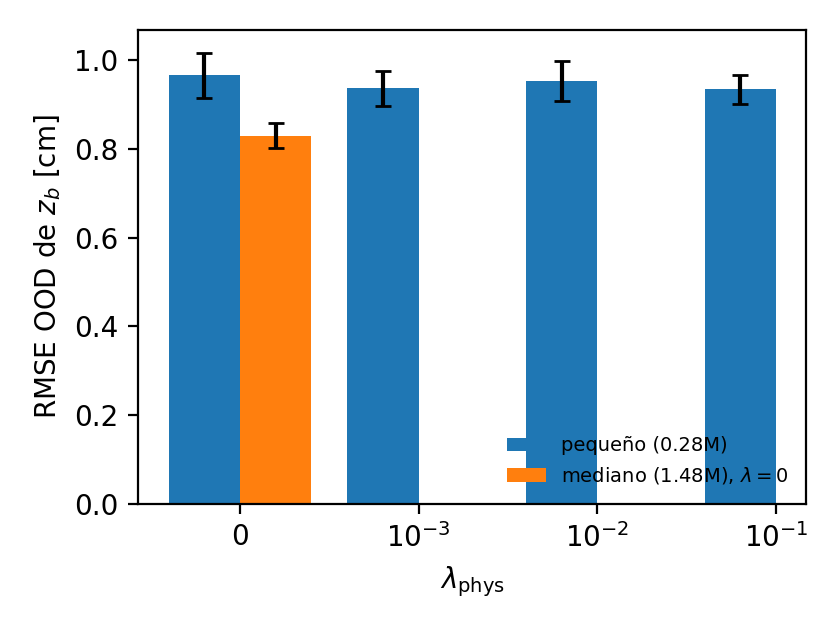
\includegraphics[width=\columnwidth]{figures/operator_ood_bars.png}
\caption{$\RMSE$ OOD (media$\pm$desv.\ est.) del operador pequeño por peso
físico $\lambda_{\text{phys}}$ ($5$ semillas) y del mediano supervisado
($\lambda_{\text{phys}}=0$, $3$ semillas, preliminar). El peso físico reduce
levemente el error del pequeño; el mediano queda por debajo de todas las
configuraciones del pequeño.}
\label{fig:bars}
\end{figure}

\subsection{Generalización acotada por la dificultad}
El error crece de forma monótona con el \emph{score} de dificultad (correlación
de Spearman $\rho\approx0.53$, $p<10^{-3}$, sobre los $15\,000$ casos OOD de las
$5$ semillas). La Fig.~\ref{fig:cliff} lo muestra: el error es estable hasta un
score $\approx 0.57$ y luego sube de forma abrupta; el decil más difícil tiene
$\approx 5.5\times$ el error del más fácil ($16.4$ vs $3.0$\,mm). Este
``acantilado'' lo causa la complejidad espacial (muchos relieves angostos), no
la emergencia del fondo (excluida por diseño). Las curvas con y sin término
físico se superponen, de modo que la leve mejora del regularizador actúa de
forma pareja sobre todo el rango y no rescata específicamente la cola difícil.

\begin{figure}[t]
\centering
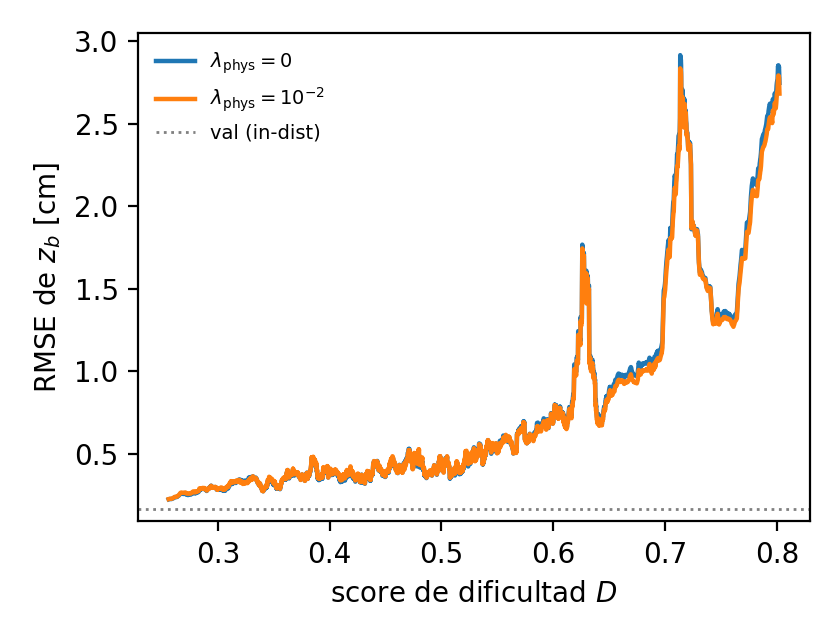
\includegraphics[width=\columnwidth]{figures/error_vs_score.png}
\caption{$\RMSE$ medio por caso vs.\ \emph{score} de dificultad en el test OOD
(operador pequeño, $5$ semillas). El error es plano hasta score $\approx 0.6$ y
luego crece de forma abrupta; las curvas con y sin física se superponen. La
línea punteada marca el error in-distribution de referencia.}
\label{fig:cliff}
\end{figure}

% =====================================================================
\section{Conclusiones}
\label{sec:concl}

Planteamos la inversión de batimetría como el aprendizaje de un operador inverso
amortizado sobre una distribución de fondos, evaluado fuera de distribución por
dificultad en un banco realista de oleaje incidente en dominio abierto. El
operador invierte fondos no vistos y más difíciles que los de entrenamiento con
un $\RMSE$ de $\sim$1\,cm, una brecha de generalización de $\approx$5.7$\times$
respecto al error in-distribution. Sobre este banco, un regularizador físico
ligero (el residuo de continuidad SWE) mejora de forma modesta pero consistente
la generalización del operador pequeño ($\approx$3\%), y evidencia preliminar
indica que aumentar la capacidad también ayuda (el operador mediano generaliza
$\approx$14\% mejor); ambos efectos contrastan con bancos previos más pobres,
donde el término físico era neutro y la capacidad no rendía, lo que sugiere que
una ventana de observación más rica vuelve a ambos provechosos. El límite
dominante, sin embargo, sigue siendo la complejidad batimétrica: el error es
plano hasta un umbral de dificultad y luego se degrada de forma abrupta. Como
trabajo futuro proyectamos completar el barrido del operador mediano, la
extensión a 2D (en curso) y la inversión sobre datos reales de fiordos (campaña
ADCP de Reloncaví).

% =====================================================================
\section*{Agradecimientos}
\TODO{financiamiento / cómputo si corresponde.}

\bibliographystyle{IEEEtran}
\bibliography{references}

\end{document}
